\documentclass{article}
\usepackage[utf8]{inputenc}
\usepackage{graphicx}

\title{Rapport intermédiaire}
\author{Sriguru ELUMALAI, Lathan TARMAT}
\date{\today}

\begin{document}

\maketitle

\section{Introduction}

Le bâtiment de la Halle aux Farines de l'Université Paris Cité accueille un nombre important d'étudiants et d'enseignants chaque année. Afin de simplifier leurs déplacements au sein de cette infrastructure, le projet a pour objectif de développer une application de guidage innovante pour faciliter la navigation à l'intérieur du bâtiment universitaire, offrant ainsi une solution pratique et efficace pour les étudiants, le personnel et les visiteurs.

Pour évaluer le succès du projet, il est essentiel de définir une métrique claire et pertinente. Dans notre cas, la métrique de succès est définie par la précision de la localisation des utilisateurs et l'efficacité du guidage fourni par l'application. En d'autres termes, le projet sera considéré comme un succès si l'application est capable de localiser les utilisateurs avec précision et de leur fournir des instructions de navigation fiables à l'intérieur du bâtiment.

Dans les sections suivantes de ce rapport, nous détaillerons l'approche technique adoptée pour la mise en œuvre du projet, les progrès réalisés jusqu'à présent, ainsi que les défis rencontrés et les solutions envisagées. Nous examinerons également les tâches restantes à accomplir pour mener le projet à sa conclusion, ainsi que les prochaines étapes prévues pour le développement de l'application de guidage.

\section{Implémentation}

\subsection{Architecture Technique}

\subsubsection{Composants Matériels}
\begin{enumerate}
    \item ESP32 (Borne de Localisation) : Déployés stratégiquement dans le bâtiment pour détecter les tags de localisation portés par les utilisateurs.
    \item ESP32 (Tag de Localisation) : Portés par les utilisateurs pour émettre des signaux détectables par les bornes de localisation, permettant de déterminer leur position.
\end{enumerate}

\subsubsection{Composants Logiciels}
\begin{enumerate}
    \item Serveur Node.js : Gère la communication entre les composants matériels et logiciels, reçoit les données de localisation, effectue la triangulation et transmet les informations à l'interface web.
    \item Interface Web (Client) : Permet aux utilisateurs de saisir leur destination, affiche les instructions de navigation fournies par le serveur et communique pour calculer les itinéraires les plus courts.
\end{enumerate}

\subsubsection{Stockage de Données}
Utilisation d'un fichier CSV pour stocker les données relatives à la structure du graphe de navigation à l'intérieur du bâtiment, utilisé par le serveur pour calculer les itinéraires de navigation optimaux.


\begin{figure}[h!]
    \centering
    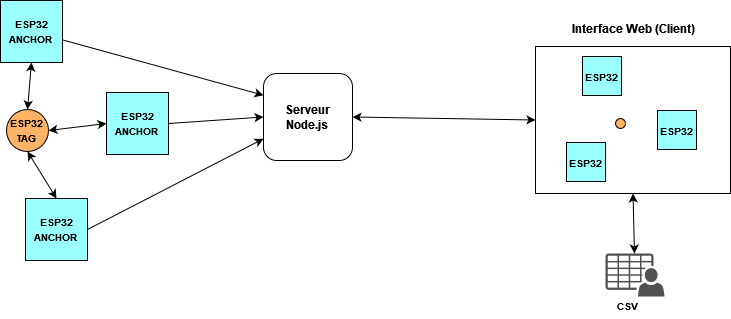
\includegraphics[width=0.8\textwidth]{architecture_globale.png}
    \caption{Architecture technique}
    \label{fig:architecture}
\end{figure}

\subsection{Fonctionnalités Développées}

À ce stade du projet, plusieurs fonctionnalités clés ont été développées :
\begin{itemize}
    \item \textbf{Affichage des étages :} Intégration de plans vectoriels SVG pour chaque étage du bâtiment dans l'interface web de l'application, offrant ainsi une représentation visuelle claire et précise de la disposition spatiale des lieux.
    \item \textbf{Modélisation des étages en graphe :} Modélisation du plan de chaque étage sous forme d'un graphe, où les nœuds représentent les points de repère importants (par exemple, les portes des salles et les intersections) et les arêtes représentent les chemins entre ces points.
    \item \textbf{Algorithme de Dijkstra :} Implémentation de l'algorithme de Dijkstra sur le serveur pour calculer les chemins de navigation optimaux entre les différents points du graphe.
    \item \textbf{Simulateur de Données de Localisation :} Développement d'un simulateur en Python pour générer des données simulées de localisation en attendant la disponibilité du matériel de localisation requis (ESP32).
    \item \textbf{Algorithme de Triangulation :} Mise en place d'un algorithme de triangulation sur le serveur pour estimer la position des utilisateurs en fonction des signaux reçus par les dispositifs de localisation.
\end{itemize}


\subsection{Technologies Utilisées}

Nous avons utilisés une combinaison de technologies pour le développement de l'application :
\begin{itemize}
    \item NodeJS : Utilisé pour le développement du serveur.
    \item Python : Utilisé pour le développement du simulateur de données de localisation.
    \item PHP, HTML, CSS, JavaScript : Utilisés pour le développement de l'interface utilisateur web.
\end{itemize}

\section{Jalons}

Le projet est divisé en plusieurs tâches, chacune représentant une étape clé dans le développement de l'application de guidage.

\begin{itemize}
    \item \textbf{Octobre :} (1) Définir les spécifications détaillées du projet.
    \item \textbf{Novembre :} (2) Modélisation des étages du bâtiment, (3) Recherche sur les technologies radio et capteurs de distance.
    \item \textbf{Décembre :} (4) Implémentation de la première interface web.
    \item \textbf{Janvier :} (5) Modélisation des étages en graphe, (6) Mise en place du stockage de données, (7) Affichage de la position de l’utilisateur et des bornes sur un étage.
    \item \textbf{Février :} (8) Extensions des fonctionnalités de recherche du plus court chemin, (9) Amélioration de l'interface graphique.
    \item \textbf{Mars :} (10) Recherche d'un simulateur Arduino, (11) Intégration et tests de communication, (12) Amélioration de l'algorithme de triangulation.
    \item \textbf{Avril :} (13) Amélioration de l’interface de la page web, (14) Tests approfondis, (15) Finalisation de l'application.
    \item \textbf{Mai :} (16) Présentation du projet.
    
 
\begin{figure}[h!]
    \centering
    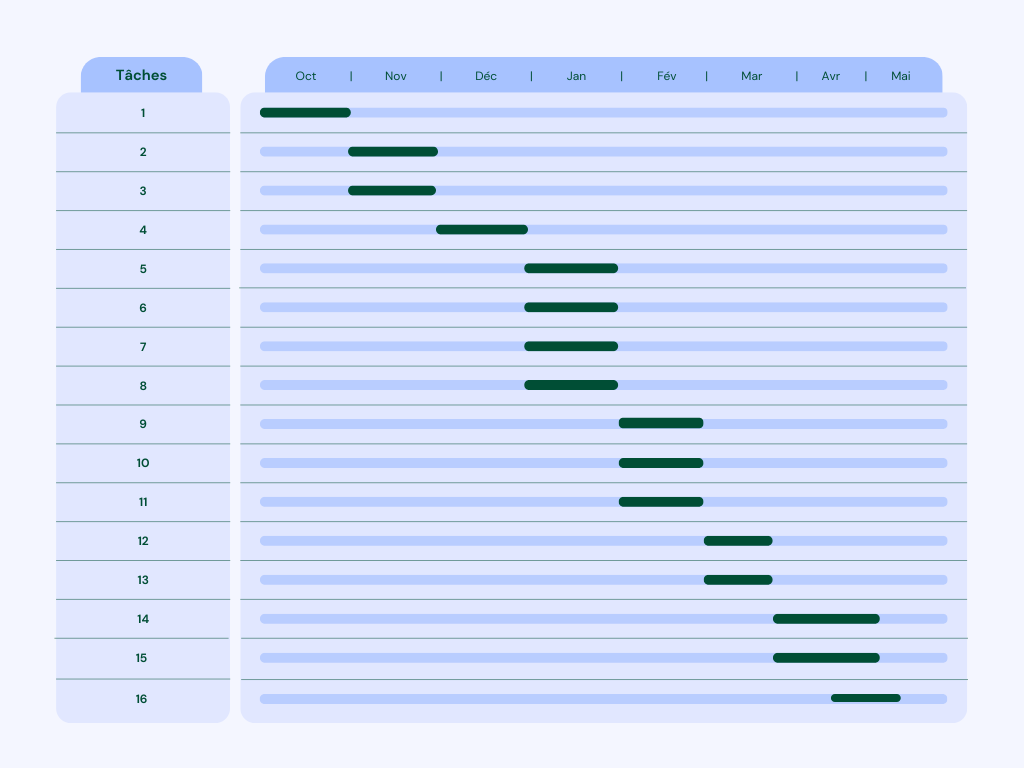
\includegraphics[width=0.8\textwidth]{Jalon.png}
    \caption{Jalons du projet}
    \label{fig:jalons}
\end{figure}

\end{itemize}



\section{Défis rencontrés et Solutions Envisagées}

Au cours du développement de l'application de guidage, plusieurs défis ont été rencontrés :

\begin{itemize}
    \item Simulation de la triangulation sans le matériel de localisation requis (ESP32), résolue par le développement d'un simulateur de données en Python pour valider les fonctionnalités de localisation.
    
    \item Recherche de fournisseurs pour l'acquisition de l'ESP32 UWB ou d'une alternative appropriée pour le matériel de localisation, crucial pour assurer le bon fonctionnement de l'application.
    
    \item Abandon inattendu du binôme de projet (Lathan TARMAT), entraînant une réorganisation immédiate des responsabilités et une augmentation de la charge de travail pour maintenir la progression du projet.
\end{itemize}


\section{Conclusion}

En conclusion, ce rapport intermédiaire souligne les progrès réalisés dans le développement de l'application de guidage pour le bâtiment de la Halle aux Farines de l'Université Paris Cité. Il reste à mettre en place l'intégration des dispositifs de localisation ESP32 avec leurs communications au serveur, améliorer l’interface de la page web et mener des tests approfondis de l'application pour détecter et corriger les éventuels problèmes.

\end{document}

